\documentclass[a4paper,10pt]{article}

\usepackage{amsmath}
\usepackage{color}
\usepackage{IEEEtrantools}
\usepackage{graphicx}

\newenvironment{meta}[0]{\color{red} \em}{}

%opening
\title{Notes on Testing and Extensions to the Rao-Blackwellised Particle Smoother}
\author{Pete Bunch}

\begin{document}

\maketitle

\section{Comparison of RB Particle Smoothers}

We have four RB smoothing algorithms for comparison: the filter-smoother (result of the final frame of the RB particle filter), the Kim's approximation smoother (which ignores the linear state contribution), the linear sampling smoother (of Fong et al.), and the full smoother (of Sarkka et al.). Previous tests have shown negligible difference between these.

\subsection{The Model}

The following model has been used for comparing the algorithms. It has been invented purely for this test and has limited physical meaning. A particle moves in one dimensions, and experiences a stochastic excitation of its $(d-1)$th derivative. All the derivatives are subject to a mean reversion effect to ensure stability.
%
\begin{IEEEeqnarray}{rClR}
 dz^{(d-1)}(t) & = & -\lambda_{d-1} z^{(d-1)}(t)dt + \sigma d\beta(t) & \\
 dz^{(n)}(t) & = & (z^{(n+1)} - \lambda_n z^{(n)})dt & 0 \le n < d-1
\end{IEEEeqnarray}

Stack this lot up into a matrix equation.
%
\begin{IEEEeqnarray}{rCl}
 x(t) &=& \begin{bmatrix} z(t) \\ z'(t) \\ \vdots \\ z^{(d-1)} \end{bmatrix}
\end{IEEEeqnarray}
\begin{IEEEeqnarray}{rCl}
 dx(t) &=& \begin{bmatrix} -\lambda_0 & 1 & \dots & 0 & 0 \\
                           0 & -\lambda_1 & \dots & 0 & 0 \\
                           \vdots & \vdots & \ddots & \vdots & \vdots \\
                           0 & 0 & \dots & -\lambda_{d-2} & 1 \\
                           0 & 0 & \dots & 0 & -\lambda_{d-1} \end{bmatrix}
 x(t) dt + \begin{bmatrix} 0 \\ 0 \\ \vdots \\ \sigma \end{bmatrix} d\beta(t)
\end{IEEEeqnarray}

This is easily discretised by matrix fraction decomposition.
%
\begin{IEEEeqnarray}{rCl}
 x_k = A x_{k-1} + w_k
\end{IEEEeqnarray}

$w_k$ is a Gaussian random variable with covariance $Q_n = \sigma^2 Q$ where $Q$ is constant (for fixed size time step).

Now to make it only conditionally linear-Gaussian. We'll make $\sigma^2$ variable over time. The ``nonlinear'' part of the state will be modelled as a first order AR process driven by Gaussian noise.
%
\begin{IEEEeqnarray}{rCl}
 u_k = \alpha u_{k-1} + \epsilon_k
\end{IEEEeqnarray}

$\epsilon_k$ is a Gaussian random variable with covariance $\Psi$ (constant for fixed size time step).

Now make $\sigma_k^2 = u_k^2$. Finally, we make linear-Gaussian observations of the $z_k$ only.
%
\begin{IEEEeqnarray}{rCl}
 y_k = C z_{k} + v_k
\end{IEEEeqnarray}
\begin{IEEEeqnarray}{rCl}
 C = \begin{bmatrix}1 & 0 & \dots & 0 \end{bmatrix}
\end{IEEEeqnarray}
\begin{IEEEeqnarray}{rCl}
 v_k \sim \mathcal{N}(v_k|0,R)
\end{IEEEeqnarray}

To summarise, our dynamics are specified by the following equations.
%
\begin{IEEEeqnarray}{rCl}
 u_k &=& \alpha u_{k-1} + \epsilon_k \\
 \epsilon_k &\sim& \mathcal{N}(\epsilon_k|0, \Psi) \\
 \sigma_k^2 &=& u_k^2 \\
 x_k &=& A x_{k-1} + w_k \\
 w_k &\sim& \mathcal{N}(w_k|0, \sigma_k^2 Q) \\
 y_k &=& C x_k + v_k \\
 v_k &\sim& \mathcal{N}(v_k|0, R)
\end{IEEEeqnarray}

This nicely fits the conditionally linear-Gaussian framework required for RB filtering and smoothing. It is also easy to vary the number of state dimensions, $d$ to test the effect on algorithm performance.



\section{Testing}

Here are some results, using 100/10 filter particle and 100/10 smoother trajectories on 5000 time steps, with 1 -- 10 dimensions.

%\begin{table}[!h]
%\centering
%\scriptsize
%\begin{tabular}{|c|c|c|c|c|c|c|c|c|c|c|}
%\hline
%                & \multicolumn{10}{|c|}{RMSE} \\
%Algorithm       & d = 1  & d = 2  & d = 3  & d = 4  & d = 5  & d = 6  & d = 7  & d = 8  & d = 9  & d = 10 \\
%\hline
%Filter-smoother & 0.2063 & 0.2257 & 0.2438 & 0.2468 & 0.2754 & 0.2780 & 0.2869 & 0.2927 & 0.2749 & 0.2685 \\
%Kim's approx.   & 0.1552 & 0.1722 & 0.1871 & 0.2060 & 0.1954 & 0.2223 & 0.2188 & 0.2337 & 0.2204 & 0.2271 \\
%Linear-sampling & 0.1573 & 0.1728 & 0.1859 & 0.2020 & 0.1893 & 0.2139 & 0.2073 & 0.2245 & 0.2087 & 0.2048 \\
%Full            & 0.1567 & 0.1714 & 0.1880 & 0.2049 & 0.1896 & 0.2136 & 0.2059 & 0.2250 & 0.2076 & 0.2035 \\
%\hline
%\end{tabular}
%\caption{RMSEs from smoothers using 100 filter particles and 100 smoother trajectories.}
%\label{}
%\end{table}
%
%\begin{table}[!h]
%\centering
%\scriptsize
%\begin{tabular}{|c|c|c|c|c|c|c|c|c|c|c|}
%\hline
%                & \multicolumn{10}{|c|}{RMSE} \\
%Algorithm       & d = 1  & d = 2  & d = 3  & d = 4  & d = 5  & d = 6  & d = 7  & d = 8  & d = 9  & d = 10 \\
%\hline
%Filter-smoother & 0. & 0. & 0. & 0. & 0. & 0. & 0. & 0. & 0. & 0. \\
%Kim's approx.   & 0. & 0. & 0. & 0. & 0. & 0. & 0. & 0. & 0. & 0. \\
%Linear-sampling & 0. & 0. & 0. & 0. & 0. & 0. & 0. & 0. & 0. & 0. \\
%Full            & 0. & 0. & 0. & 0. & 0. & 0. & 0. & 0. & 0. & 0. \\
%\hline
%\end{tabular}
%\caption{RMSEs from smoothers using 10 filter particles and 10 smoother trajectories.}
%\label{}
%\end{table}

\begin{figure}[!h]
\centering
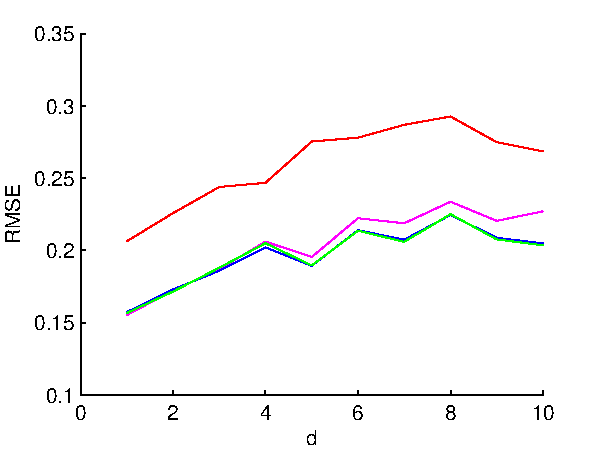
\includegraphics[width=0.9\columnwidth]{RMSE_comparison100.pdf}
\caption{RMSEs for filter-smoother (red), Kim's approximation smoother (pink), linear-sampling smoother (blue), full smoother (green) using 100 filter particle and 100 smoother trajectories.}
\end{figure}

\begin{figure}[!h]
\centering
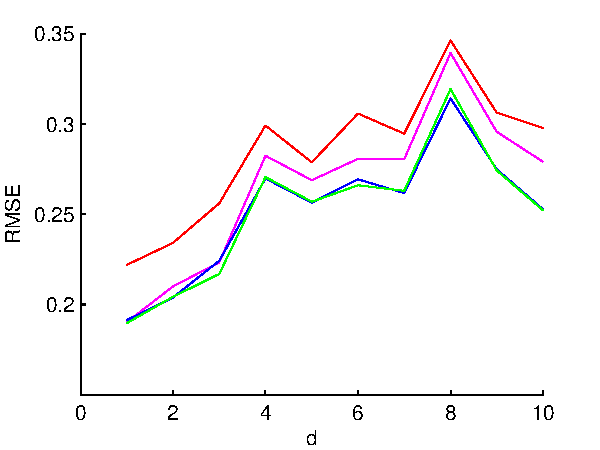
\includegraphics[width=0.9\columnwidth]{RMSE_comparison10.pdf}
\caption{RMSEs for filter-smoother (red), Kim's approximation smoother (pink), linear-sampling smoother (blue), full smoother (green) using 10 filter particle and 10 smoother trajectories.}
\end{figure}

It looks like we can conclude that the Kim's approximation smoother deteriorates with the dimension of the linear state, and that all of them outperform the filter-smoother (i.e. Kitagawa smoother). However, there's no significant difference between the linear-sampling (Fong et al.) and full (Sarkka et al.) smoothers on this test.

Additionally, a second model has been tried in which there is an independent driving Brownian motion on every derivative, all with the same standard deviation, $sigma_k$, so the dimension of $w_k$ is also $d$. RMSE results closely resemble those above with a single Brownian motion.



\section{Other Testing}

Tests have also been conducted using a different model, in which a number of Brownian motion or Ornstein�Uhlenbeck processes are run in parallel, conditional upon a common, time-varying diffusion constant (the ``nonlinear'' part of the state) which evolves according to an AR process. Testing using a wide variety of model and algorithm parameters yielded no combination for which the full smoother outperformed the linear-sampling smoother. 



\section{MCMC smoothing}

The new MCMC smoothing algorithms can be applied to conditionally linear-Gaussian models.

At the moment, we're sampling the conditional distribution (or an approximation thereof),  $p(u_{1:k}|u_{k+1:K}, y_{1:K})$, directly. This means that we have to calculate a sampling weight for each filtering particle at every time step for every smoothing trajectory, so the complexity is $\mathcal{O}(N_F \times N_S \times K)$. We could bring this down using MCMC with a short chain, instead of direct sampling. Briefly, a new nonlinear sequence, $u_{1:k}^*$, is proposed from the particle approximation of $p(u_{1:k}|y_{1:k})$ which we already have from the filter. This is accepted with probability,

\begin{IEEEeqnarray}{rCl}
 \alpha &=& \left[ 1, \frac{p(u_{1:k}^*|u_{k+1:K}, y_{1:K}) p(u_{1:k}|y_{1:k})}{p(u_{1:k}|u_{k+1:K}, y_{1:K}) p(u_{1:k}^*|y_{1:k})} \right] \\
  &=& \left[ 1, \frac{ \int p(y_{k+1:K}|x_k, u_{1:k}^*, u_{k+1:K}) p(x_k|u_{1:k}^*, y_{1:k}) dx_k p(u_{k+1}|u_k^*) }{ \int p(y_{k+1:K}|x_k, u_{1:k}, u_{k+1:K}) p(x_k|u_{1:k}, y_{1:k}) dx_k p(u_{k+1}|u_k) } \right]     .
\end{IEEEeqnarray}

Using this strategy, we only calculate ``weights'' of the particles we actually visit. Accuracy approaches that of the direct sampler as the length of the chain, $M$, increases. As long as $M<N_F$, then this is quicker than direct sampling.

We can extend this framework to construct a smoother which is not limited to the support of the filtering approximation. We can expand the target distribution as,
%
\begin{IEEEeqnarray}{rCl}
 p(u_{1:k}|u_{k+1:K}, y_{1:K}) & \propto & \int p(y_{k:K}|x_k, u_{1:k}, u_{k+1:K}) p(x_k|u_{1:k}, y_{1:k-1}) dx_k \nonumber \\
  & & \times p(u_{k+1}|u_k) p(u_{k}|u_{k-1}) p(u_{1:k-1}|y_{1:k-1})     .
\end{IEEEeqnarray}

Now we can change the MCMC proposal to $p(u_{1:k-1}|y_{1:k-1}) q(u_k|u_{k-1}, u_{k+1}, y_{1:K})$. The corresponding acceptance probability is,
%
\begin{IEEEeqnarray}{rCl}
 \alpha &=& \left[ 1, \frac{p(u_{1:k}^*|u_{k+1:K}, y_{1:K}) p(u_{1:k-1}|y_{1:k-1}) q(u_k|u_{k-1}, u_{k+1}, y_{1:K})}{p(u_{1:k}|u_{k+1:K}, y_{1:K}) p(u_{1:k-1}^*|y_{1:k-1}) q(u_k^*|u_{k-1}, u_{k+1}, y_{1:K})} \right] \\
  &=& \left[ 1, \frac{ \int p(y_{k:K}|x_k, u_{1:k}^*, u_{k+1:K}) p(x_k|u_{1:k}^*, y_{1:k-1}) dx_k }{ \int p(y_{k:K}|x_k, u_{1:k}, u_{k+1:K}) p(x_k|u_{1:k}, y_{1:k-1}) dx_k } \right. \nonumber \\
  & & \qquad \left. \frac{ p(u_{k+1}|u_k^*) p(u_{k}^*|u_{k-1}) q(u_k|u_{k-1}, u_{k+1}, y_{1:K}) }{ p(u_{k+1}|u_k) p(u_{k}|u_{k-1}) q(u_k^*|u_{k-1}, u_{k+1}, y_{1:K}) } \right]     .
\end{IEEEeqnarray}

The difficulty here would be devising good choices for $q(u_k|u_{k-1}, u_{k+1}, y_{1:K})$, which will be significantly more complex than the standard (i.e. not RB) case.



\end{document} 